\section{Results}
\label{sec:results}
This section presents an evaluation of our results and a discussion of the model's performance. We begin with a visual comparison between an estimated and ground-truth pose, followed by a detailed analysis of the model's performance on the test set. Finally, we examine the resulting trajectories from our localization pipeline.

\subsection{Visual comparison of estimated and ground truth pose}
Figure \ref{fig:pose-comparison} illustrates a visual comparison between the estimated pose and the corresponding ground truth from the test set, shown from four perspectives rotated at 0°, 90°, 180° and 270° angles. Overall, the estimated pose captures the global body posture of the target well. In particular, the global orientation of the skeleton and the left-leg joint positions align closely with the ground truth. However, discrepancies are visible in the right lower leg, which appears shifted further back relative to the ground truth. Furthermore, the estimated upper body exhibits a slightly stronger forward lean that the reference.

\begin{figure}[htbp]
    \centering
    \includegraphics[width=\columnwidth]{img/pose_comparison.pdf}
    \caption{Comparison of a single estimated pose (red) to its ground truth pose (blue) from different perspectives.}
    \Description{}
    \label{fig:pose-comparison}
\end{figure}

\subsection{Metrics}

\subsection{Localization and Kalman-Filter Effect}
In \ref{subsec:localization}, we introduced our approach for extracting information about the person's current global position from the SensFloor activation signals. The left side of Figure \ref{fig:kalman-filter-effect} shows the raw clustering position trajectory we recorded during a test walk. The illustrated trajectory is highly erratic. This instability is caused by two main factors. First, the algorithm creates jumpy in the estimated position as the mean shifts abruptly whenever a foot makes or breaks contact with the floor. Second, the SensFloor fields produce significant background noise, even in areas where no activity takes place. While increasing the noise signal threshold suppresses some of the noise, it is not a universal solution, as signal intensity of people moving on the floor varies depending on the person's footwear. 

However, applying the Kalman filter largely reduces these issues, as illustrated on the right side of Figure \ref{fig:kalman-filter-effect}. By smoothing out the abrupt transitions and mitigating the impact of outliers, the filter produces a smooth and, according to our empirical evaluation, accurate trajectory.

\begin{figure}[htbp]
    \centering
    \includegraphics[width=\columnwidth]{img/kalman-filter-effect.pdf}
    \caption{To-do}
    \Description{}
    \label{fig:kalman-filter-effect}
\end{figure}

% - Predicted pose compared to true pose image
% - Training metrics (boxplot and mention pck) explain tha numbers
% - Estimated position (House of Kalmann)
% - Inference works